%==================================
\chapter{Architectural Description}
%==================================
This chapter introduces the architectural documents pertaining to our solution. The team followed the definition of software architecture defined by Len Bass, Paul Clements and Rick Kazman: "The software architecture of a program or computing
system is the structure of structures of the system, which comprise software elements, the externally visible properties of those elements, and the relationships between them."

The purpose of this document is to describe our architecture in a structured way so that it can be used not only by the team, but also as an aid for other stakeholders who are trying to understand the system.

\section{Architectural Drivers}
%------------------------------
This section is dedicated to the discussion of the architectural drivers
The team has chosen Modifiability and Testability as the quality attributes for this utility. 

The reason for using Modifiability is that the development team are not going to be the ones updating or maintaining the utility after the completing the project. It is therefore important that the code is easy to understand, good documented and easy to modify. This will make it easier for our customer to later modifiy or extend the utility.

Testability is important since the utility will be used for debugging by the customer.  Since it is not possible for the team to test the dissectors in a real enviorment, it will be more important to focus on testing. This to ensure that the final product is working correctly.

\subsection{Testability Tactics}
The goal of using testability tactics is making it easier to test the system after finishing an increment of the software development. 

\subsubsection{Specialize access routes/interfaces}
Using a specialized testing interface makes it possible to specify values for a component independently from its normal execution. This will in turn make it possible to test parts of an unfinished module as well as making it easier to get a clear overview over what data is flowing through individual parts of the system.

\subsection{Modifiability Tactics}
The goal of using modifiability tactics are to make it easier to extend and modify the software during the development and after having made a working product.

\subsubsection{Anticipate Expected Changes}
By trying to anticipate expected changes it is possible to make it easier for modules to be extended with new functionality later. It also makes it easier for the developers to anticipate the different ranges of input the modules are about be able to process.

\subsubsection{Limit Possible Options}
By limiting the range of possible modifications to the system it becomes easier to generalize the structure of different modules. This will in turn make it easier to constrict the wide ranging effect of new modifications to the system, giving the developers a clearer view over what a given change will actually do to the system.

\subsubsection{Generalizing Modules}
Generalizing the modules of a system makes it possible to reuse older modules when doing modifications to the system. The more general a module, the more likely it is that a needed change to the system can be implemented just by adjusting the input to the system rather than having to modify existing or creating new modules.

\subsubsection{Restrict Communication Paths}
By restricting the number of modules that are able to collect data from a specific module, the less dependent the entire system becomes of that specific module. This makes it easier to swap out existing modules with new ones without having to make many widespread changes to the entire system.

\subsubsection{Using Configuration Files}
By using configuration files, it is possible to change the behaviour of the system without having to do any changes to its code.

\subsection{Business Requirements}


\section{Architectural Patters}
%------------------------------
This section presents the different architectural patterns used in the utility
\subsection{Pipe and Filter}
The pipe and filter architectural pattern consists of a stream of data which is in turn processed sequentially by several filters in such a fashion that the output of one filter becomes the input of the other. It is a very flexible yet robust way of processing data, with support for adding more filters if needed for future applications and processes.
\begin{figure}[ht]
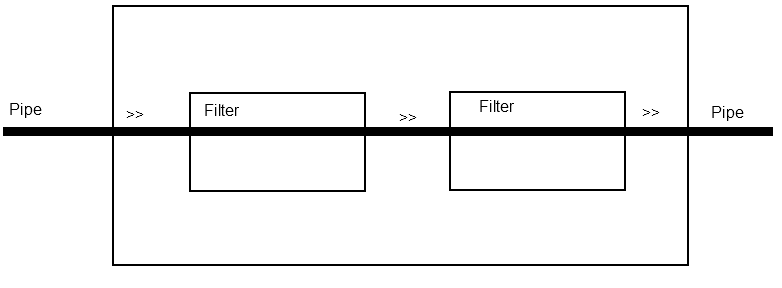
\includegraphics[width = \textwidth]{./planning/img/PipeAndFilter}
\caption{Pipe and Filter Pattern} 
\label{fig:pipefilter}
\end{figure}

\section{Architectural Views}

\subsection{Logical View}
This view shown in \autoref{fig:logicalview}. Command line takes the arguments for header file and configuration file as a string. The arguments are parsed in the command line parser. Header file is sent to ''C preprocessor \& C parser", the c header file is loaded and parsed by the c parser, and generate a parsing tree. Command line also call Configuration, which load the configuration file. The configuration will parse the configuration file and create configuation rules. The Lua script generator will generate a Lua script from the parseing tree and the config rules.

\begin{figure}[ht]
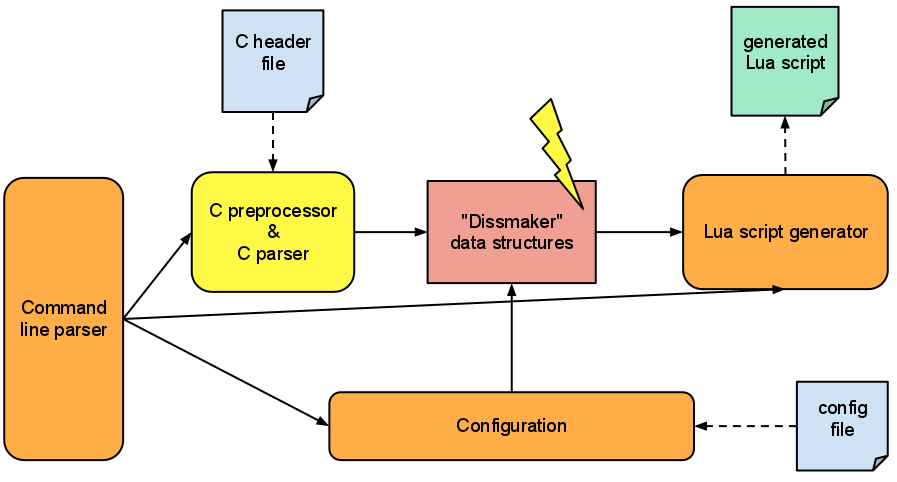
\includegraphics[width=\textwidth]{./planning/img/overall_design.png}
\caption{Overall Architecture}
\label{fig:logicalview}
\end{figure}

\section{Process View}


\section{Deployment View}

\section{Architectural Rationale}
%--------------------------------

